%{{{ prelude latex
\tracingmacros=0
\documentclass[a4paper]{article}

%{{{ packages
\usepackage[colorlinks]{hyperref}
\usepackage{amsmath}
\usepackage{amssymb}
\usepackage{amsthm}
\usepackage{listings}
\usepackage{mathrsfs}
\usepackage{microtype}
\usepackage{rgalg}
\usepackage{slemph}
\usepackage[center]{subfigure}
\usepackage{tikz}
\usepackage{xcolor}
\usepackage{xspace}
\usepackage{hyperref}  % solves pdfTeX warning (ext4)?
\usepgflibrary{arrows}
\usepgflibrary{shapes.geometric}
%}}}
%{{{ PDF settings
\definecolor{darkblue}{rgb}{0,0,0.4}
\definecolor{verylightgray}{rgb}{0.9,0.9,0.9}
% comment the next line for printing
\hypersetup{colorlinks,linkcolor=darkblue,citecolor=darkblue,urlcolor=darkblue}
\hypersetup{
  pdfauthor={Mikol\'a\v{s} Janota and Radu Grigore},
  pdftitle={Semantic Reachability}}
%}}}
%{{{ tikz helpers

% global styles
\tikzstyle{arr}=[->,>=stealth']
\tikzstyle{predcirc}=[
  circle,
  very thick,
  fill=green!10,
  draw=green,
  minimum size=14pt,
  inner sep=0pt]
\tikzstyle{predrect}=[predcirc,rectangle,inner sep=2pt]

% These macros and styles are used for drawing flowgraphs
\newcommand\fgnodeR{2pt}  % the default radius of a flowgraph node
\tikzstyle{fgdraw}=[
  minimum size=2*\fgnodeR,inner sep=0pt,outer sep=1pt,
  draw,thick]
\tikzstyle{fgfill}=[fill=black]
\ifx\fgnode\undefined\else\errmessage{\string\fgnode already defined!}\fi
\def\fgnode#1#2(#3) at (#4){% uses \def because of the special syntax
    \begin{scope}[shift={(#4)},shift only]
      \clip (-\fgnodeR,-#1*\fgnodeR) rectangle (\fgnodeR,#2*\fgnodeR);
      \node[fgdraw,circle,fgfill] {};
    \end{scope}
    \node[fgdraw,circle] (#3) at (#4)}
\newcommand{\oonode}{\fgnode00} % the normal non-reading non-writing node
\newcommand{\ronode}{\fgnode01} % for read-only nodes
\newcommand{\wonode}{\fgnode10} % for write-only nodes
\newcommand{\rwnode}{\fgnode11} % for read-write nodes
\newcommand{\gnode}{\node[fgdraw,circle,fill=gray]}  % gray nodes (ra)
\newcommand{\cnode}{\node[fgdraw,fgfill,rectangle]} % copy nodes
\newcommand{\enode}{\oonode} % empty node
\newcommand{\fnode}{\rwnode} % filled node
%}}}
%{{{ package customization
\lstset{
  basicstyle=\scriptsize,
  identifierstyle=\itshape,
  stringstyle=\footnotesize\ttfamily,
  commentstyle=\textup,
  columns=fullflexible,
  numbers=left,
  numberstyle=\tiny,
  mathescape=true,
  boxpos=t,
}
\lstdefinestyle{boogie}{
  morekeywords={procedure,returns,assume,assert,havoc,goto,return,
    int,bool,type,while,if,true,false,function,bool,returns,axiom,
    forall,var}
}
\lstdefinestyle{jml}{
  language=java,
  morekeywords={requires,ensures,old,invariant,forall,exists,axiom,also,
    result,pure,assert,modifies},
  deletekeywords={label}
}
\lstdefinestyle{smt}{
  morekeywords={ite,true,false,BG_PUSH,IFF,FORALL,EQ,NEQ,NOT,TRUE,FALSE,
    IMPLIES}
}
\newcommand{\lstinlinen}{\lstinline[basicstyle=\normalsize]}
\newcommand{\boogieCode}{\lstinline[style=boogie,basicstyle=\normalsize]}
\newcommand{\jmlCode}{\lstinline[style=jml,basicstyle=\normalsize]}
\newcommand{\smtCode}{\lstinline[style=smt,basicstyle=\normalsize]}
\newcommand{\deflang}[1]{\lstnewenvironment{#1}[1][]{\lstset{style=#1,##1}}{}}
\deflang{jml}
\deflang{boogie}
\deflang{smt}
%}}}
%{{{ new commands 
\def\fb#1{{\bf #1}}
\newcommand{\escjava}{ESC\slash Java\xspace}
\newcommand{\fls}{\bot}
\newcommand{\hoare}[3]{\{#1\}\>\text{#2}\>\{#3\}}
\newcommand{\limp}{\Rightarrow}
\newcommand{\mj}[1]{{\small [\textcolor{red}{mj}: #1]}}
\newcommand{\rg}[1]{{\small [\textcolor{red}{rg}: #1]}}
\newcommand{\todo}[1]{{\small [\textcolor{red}{TODO:} #1]}}
\newcommand{\tru}{\top}

%pairs
\newcommand{\startgrammar}{
  \begingroup
  \def\is{$\>\to$&}
  \def\|{$\mid$}
  \def\b##1{\textbf{##1}}
  \def\i##1{\textsl{##1}}
  \def\?{$^?$}
  \def\*{$^\ast$}
  \begin{figure}
  \centering
  \scriptsize
  \begin{tabular}{rl}
}
\newcommand{\stopgrammar}[2]{
  \end{tabular}
  \caption{#1}\label{#2}
  \end{figure}
  \endgroup
}

\newcommand{\bc}{\begin{figure}\centering\begin{tabular}{c}} % begin codebox
\newcommand{\ec}[2]{\end{tabular}\caption{#1}\label{#2}\end{figure}} % end codebox
%}}}
%{{{ new environments (and theorems)
\newtheoremstyle{slanted}{}{}{\slshape}{}{\bf}{.}{.5em}{}
\theoremstyle{slanted}
\newtheorem{problem}{Problem}
\newtheorem{conjecture}{Conjecture}
\newtheorem{lemma}{Lemma}
\newtheorem{proposition}{Proposition}
\newtheorem{theorem}{Theorem}
\newtheorem{corollary}{Corollary}
\theoremstyle{definition}
\newtheorem{definition}{Definition}
\newtheorem{example}{Example}
\theoremstyle{remark}
\newtheorem{remark}{Remark}
%}}}
%{{{ TeX settings
\overfullrule=5pt
\showboxdepth=10
\showboxbreadth=100
%}}}
%{{{ metadata
\title{Semantic Reachability}
\author{Mikol\'a\v{s} Janota and Radu Grigore}
\date{}
%}}} metadata
%}}}

\begin{document}

\maketitle
\begin{abstract}
  \todo{Write.}
\end{abstract}

Program verifiers typically check for partial correctness or
termination, but there are other interesting analyses. This
chapter (1)~explains when and why reachability analysis is
useful, (2)~presents its theoretical underpinnings, and then
(3)~presents and analyzes algorithms that make it practical.

%{{{ sec:motivation
\section{Motivation}

Semantic reachability analysis finds four seemingly unrelated
types of problems: dead code, doomed code, inconsistent
specifications, and bugs in the frontend of the program verifier.

\subsection{Dead Code}

Figure~\ref{fig:ra-dead-code-ex} illustrates two problems.
Line~10 is dead in the standard sense; line~5 is dead only
if annotations are taken into account. 
  
\bc
\begin{jml}
static void m(int x) 
  requires x >= 0;
{
  if (x < 0)
    throw new IllegalArgumentException("x must be nonnegative");
  $\cdots$
  if (y < 1) {
    $\cdots$
    if (y > 1) {
      $\cdots$
  }}
}
\end{jml}
\ec{Dead code}{fig:ra-dead-code-ex}

Dead code analysis is standard in compilers. Java, for example,
forbids any statement following the statement \textbf{return},
because such situations are usually unintended bugs. The novelty
here is that we take into account annotations, which may be
non-executable. When the precondition holds (line~2) the first
\textbf{if} condition (line~4) does not, so no exception is
thrown.

In current practice, programmers check arguments at the beginning
of the method body with a series of guarded \textbf{throw}
statements. The pattern is so common that it is encapsulated in
libraries~\cite{google-collect} so that the code is slightly
shorter and slightly easier to read. The small gains add up. In
the presence of annotations, however, the code that checks if
arguments are legal is mostly redundant.

If all calls to method~$m$ are checked statically against its
specification, then no runtime check is necessary. A runtime
check remains desirable when unverified code may call method~$m$.
There are Java compilers~\cite{burdy2005jml} that generate
bytecode from JML annotations. The translation is not perfect.
One technical problem is that JML preconditions do not have
descriptions. If the expression is particularly simple (such as
$x\ge0$ in Figure~\ref{fig:ra-dead-code-ex}) then it is possible
to construct the description automatically (``$x$~must be
nonnegative''). For longer expressions, though, the automatically
generated description is unwieldy and unuseful. The problem is
just technical since it has the simple solution of modifying
JML to have descriptions for preconditions, postconditions, and
assertions. The second problem is more serious. If the expression
contains quantifiers, which in JML are typically over very large
domains like the integers, then it is not always possible to
check it efficiently at runtime. However, in such situations it
is likely that the programmer would have not written a runtime
check.


\subsection{Doomed Code}

Figure~\ref{fig:ra-doomed-code-ex} illustrates two problems, one
on line~7 and one on line~14. These where the most common issues
in practice (Section~\ref{sec:ra.case_study}).

%{{{fig:ra-doomed-code-ex
\bc
\begin{jml}
abstract class C {
  int f, g;
  static void m1(C x) {
    if (x != null)
      x.f = 0;
    else
      System.out.println(x.f);
  }
  static void m2();
    modifies f, g;
  static void m3()
    modifies f;
  {
    m2();
    $\cdots$
  }
}
\end{jml}
\ec{Doomed code}{fig:ra-doomed-code-ex}
%}}}

Execution always crashes at line~7, before printing. Any test
that covers line~7 would detect the problem, but test suites
rarely have complete coverage. The example is adapted from
Hoenicke et al.~\cite{hoenicke2009}, whose example is in turn
inspired by an old bug in Eclipse. Such bugs do occur in real
software even if they are easy to detect. It would therefore
be beneficial to find such problems automatically and without
writing any test. (But this is true about any kind of bug.)
Another reason given by Hoenicke et al.~\cite{hoenicke2009} is
compelling: \emph{The lack of annotations does not lead to false
positives}. Most frequent complaints from practicians about
formal methods tools are that
\begin{enumerate}
\item it is too much work to add annotations and
\item there are too many false positives.
\end{enumerate}
To be more precise, the lack of \emph{assumptions} (stemming,
for example, from the lack of preconditions and object
invariants) does not lead to false positives. A program point is
\emph{doomed} if it crashes in every execution. If an assumption
is removed (which may mean, for example, that more values are
allowed for an argument), then all the old executions are still
possible. In other words, removing an assumption never turns a
non-doomed program point into a doomed program point.

Line~14 is also doomed, this time because of annotations, not
because of the code. The \textbf{modifies} clause lists the
fields that a method is allowed to assign to. From the point of
view of the program verifier the execution never proceeds past
line~14, so all potential bugs that follow are hidden.

\subsection{Inconsistent Specifications}

Figure~\ref{fig:ra-bad-spec-ex} illustrates two problems caused
entirely by specifications.

%{{{fig:ra-bad-spec-ex
\bc
\begin{jml}
pure static native int m1()
  ensures result == result + 1;
static int m2(int x)
  requires x < 0;
  requires x > 0;
{
  return x / 0;
}
\end{jml}
\ec{Inconsistent specifications}{fig:ra-bad-spec-ex}
%}}}

The contract of method~\textit{m1} cannot possibly correspond to
a correct implementation, yet there is no implementation to check
against the contract. In this case the implementation is written
in a different language, but sometimes it is simply unavailable,
for example if it comes from a proprietary library. The example
may seem silly since no one would make the mistake to think that
some integer equals its successor. However, inconsistencies
may arise from other causes. One example is specification
inheritance: Since the conflicting annotations are in different
files it is hard for a human to notice. Another example is the
use of pure methods in specifications. The literature concerned
with tackling this latter source of inconsistencies is reviewed
in Section~\ref{sec:ra.conclusions}.

Lines 4~and~5 illustrate another type of bug caused by
inconsistent specifications. The body of method~\textit{m2} is
available and the program verifier will always report it is
correct. Without reachability analysis, the bug is caught only
if method~\textit{m2} is called. Such behavior is somewhat akin
testing, which catches bugs (only) by calling the (potentially)
buggy methods.

In practice, inconsistent specifications are common.

\subsection{Unsoundness and Bugs}

The code in Figure~\ref{fig:ra-loop-unroll}, apart from being
more than a little silly, will always crash at line~4. That is
not the issue relevant here, however. The issue is that the
problem may be missed by an unsound program verifier.

\bc
\begin{jml}
int x;
for (int i = 5; --i >= 0;)
  x = i;
x = 1 / x;
\end{jml}
\ec{Unsoundness of the frontend}{fig:ra-loop-unroll}

Again, the example might seem contrived. Why not get rid of
unsoundness in the first place instead? And why would we expect
this problem to appear often? Before answering these questions
let us see why this is indeed a problem in \escjava (with
default options). \escjava was designed primarily to be useful
to programmers and it tackled the problem of false positives
by choosing to be unsound. One example of unsoundness is that,
by default, loops are unrolled three times. This means that
all executions for which the body of the loop is executed more
than three times are considered to miraculously terminate with
success. All executions in Figure~\ref{fig:ra-loop-unroll} go
through the loop body five times so, just before executing the
loop body for the fourth time, \escjava will consider that the
execution finishes with success. This makes \escjava miss the
problem on line~4. Note that if the loop would be executed
$n$~times instead of $5$~times, where $n$~is a variable possibly
less than four, then the problem on line~4 would be caught.

We are now in a better position to answer the two questions.

First, a tool may choose to be unsound for engineering reasons.
This is not as bad as it may sound. We saw that a loop with
a variable bound instead of a constant bound does not cause
problems, and variable bounds are probably more common. Also,
this is only the default behavior. A novice user is supposed to
get rid of the errors signaled in this unsound default mode of
execution. An expert user is supposed to ask \escjava to treat
loops in a safe way. In this case, the tool usually requires more
guidance in the form of annotations. 

Second, the unsoundness might not be intended, but rather a bug.
In this guise, reachability analysis is useful as a safeguard
against buggy implementations of the program verifier itself.
It is common for good programmers to write routines that check
for complex invariants at runtime and use these routines during
development. Reachability analysis has been used in this way in
the Boogie tool from Microsoft Research under the name of ``smoke
testing''.

\subsection{An Unexpected Benefit}

Finally, in conjunction with loop invariant inference techniques,
reachability analysis detects certain non-terminating programs.
Consider the following code fragment.
\begin{jml}
for (int i = 0; i < 10; ++j) 
  sum += i;
$\cdots$
\end{jml}
It is easy to infer the loop invariant $i=0$, which contradicts
the negation $i\ge10$ of the loop condition. The code after the
loop is unreachable because the loop never terminates.
%}}} sec:motivation
%{{{ sec:boogie
\section{The Core Boogie}
\label{sec:boogie}

 From now on all programs are written in the Boogie
language, and almost all are written in a subset---the core
Boogie---defined in this section. What is `core' is relative to
the topics discussed in this dissertation.

Figure~\ref{lst:first-boogie} shows an implementation of
sequential search. After the counter~$i$ is initialized in line~2
the control goes nondeterministically to both labels $b$~and~$d$.
An execution gets \emph{stuck} if it hits an assumption that
does not hold. Since the conditions on the lines 3 and~5 are
complementary, exactly one of the two executions will continue.
(In general, the \textbf{if} statement of full Boogie may be
desugared into a \textbf{goto} statement that targets two
\textbf{assume} statements with complementary conditions.) The
\textbf{return} statement is reached only if $i \ge \mathit{vl}$
or $v[i]=u$.

%{{{ lst:first-boogie
\begin{figure}
\centering
\begin{tabular}{cc}
\begin{boogie}[boxpos=c]
procedure indexOf(u : int, v : [int] int, vl : int) returns (i : int) {
  a: i := 0; goto b, d;
  b: assume i < vl && v[i] != u;
  c: i := i + 1; goto b, d;
  d: assume !(i < vl && v[i] != u); return;
}
\end{boogie}&
\hspace{5mm}
\begin{tikzpicture}[scale=.5,baseline=0.7cm]
  \oonode (A) at (1,3)  [label=60:$a$] {};
  \oonode (B) at (0,2.5)  [label=135:$b$] {};
  \oonode (C) at (0,0.5)  [label=-135:$c$] {};
  \oonode (D) at (1,0)  [label=-60:$d$] {};

  \draw[arr] (A) -- (B);
  \draw[arr] (A) -- (D);
  \draw[arr] (B) to [bend right=30] (C);
  \draw[arr] (C) to [bend right=30] (B);
  \draw[arr] (C) -- (D);
\end{tikzpicture}
\\
\end{tabular}
\caption{Boogie program with one loop and its flowgraph}
\label{lst:first-boogie}
\end{figure}
%}}}

The high-level constructs of full Boogie (such as \textbf{if}
statements, \textbf{while} statements, and \textbf{call}
statements) can always be desugared into the core that is
formalized here. The concrete grammar of core statements
appears in Figure~\ref{grm:boogie-stmts}. The statement
\textbf{assert}~$p$ means ``when you reach this point, check that
$p$ holds.'' The statement \textbf{assume}~$p$ means ``continue
to look only at executions that satisfy~$p$.''

\startgrammar
  statement\is label\? (assignment \| assumption \| assertion \| jump) \b; \\
  label\is \i{id} \b{:} \\
  assignment\is id \b{:=} expression \\
  assumption\is \b{assume} expression \\
  assertion\is \b{assert} expression \\
  jump\is (\b{goto} id-tuple \b{}) \| \b{return} \\
  id-tuple\is \i{id} (\b, \i{id})\* \\
\stopgrammar{Syntax of core Boogie statements}{grm:boogie-stmts}

The type system of full Boogie is rich, featuring polymorphic
maps, bit vectors, and user-defined types, among others. Its
expression language is similarly rich. Unlike in the case
of statements, the VC generator implementation (henceforth
known as FreeBoogie) does not desugar types and expressions
into simpler ones. How they are treated, however, is not
novel. For the sake of the presentation, only a few types
and expressions are retained in the core, the ones in
Figure~\ref{grm:exprs-and-types}.

\startgrammar
  type\is primitive-type \| map-type \\
  primitive-type\is \b{int} \| \b{bool} \\
  map-type\is \b[ primitive-type \b] type \\
  expression\is \b( quantifier \i{id} \b: type \b{::} expression \b) \\
  expression\is unary-operator expression \| expression binary-operator expression \\
  expression\is expression \b[ expression \b] \\
  expression\is \i{id} \| literal \| \b( expression \b) \\
  quantifier\is \b{forall} \| \b{exists} \\
  unary-operator\is \b! \| \b- \\
  binary-operator\is \b+ \| \b- \| {\boldmath$<$} \| \b{==} \| \b{\&\&} \| {\boldmath$||$} \\
  literal\is \b{true} \| \b{false} \| \b0 \| \b1 \| \b2 \| \ldots \\
\stopgrammar{Syntax of core Boogie types and expressions}{grm:exprs-and-types}

The syntax for the overall structure of core Boogie programs
appears in Figure~\ref{grm:boogie}. Statements are preceded
by variable declarations, in which the variables representing
the input and the output are singled out. The keyword
\textbf{procedure} is retained from full Boogie, where a program
may contain more than one procedure and where there is also a
\textbf{call} statement. Procedures are not included in the core,
because there is nothing novel related to procedure calls in
this dissertation. The mandatory \textbf{return} statement at
the end of each body reduces the number of special cases that
need to be discussed later. FreeBoogie inserts such a statement
automatically during parsing, so the user does not have to end
all procedures with \textbf{return}.

\startgrammar
  program\is \b{procedure} \i{id} \b( arguments\? \b{) returns (} results\? \b) body \\
  arguments, results\is \i{id} \b: type (\b, \i{id} \b: type)\* \\
  body\is variable-declaration\* statement\* \b{return} \b; \\
  variable\is \b{var} \i{id} \b: type \b; \\
\stopgrammar{Structure of a (core) Boogie program}{grm:boogie}

Typechecking core Boogie is straightforward:
Figure~\ref{fig:boogie-typing} shows a representative sample of
the typing rules. The judgment $\vdash p$ means that the program
fragment~$p$ is well-typed and the judgment $\vdash p:t$ means
that the program fragment~$p$ is well-typed \emph{and} has the
type~$t$. The customary environment is omitted because it is
fixed---it consists of all the variable typings appearing at the
beginning of the program. The rules that are missing are similar
to the ones given: For example, there is a rule that says that
the expression appearing in an assumption must have the type
\textbf{bool} (analogous to rule [asrt]).

\begin{figure}
\centering
\begin{displaymath}
\begin{array}{ccc}
  \frac
    {\forall\:  1\le k\le n,\;
      \exists t,\;  (\vdash v_k : t \;\land\;
       \vdash e_k : t)}
    { \vdash v_1,\ldots,v_n \boldsymbol{:=} e_1,\ldots,e_n}
    \;\text{[asgn]}
  &&
  \frac{\vdash e : \mathbf{bool}}{\vdash \mathbf{assert}\;e}
    \;\text{[asrt]}
  \\ \\
  \frac
    {\vdash e : \mathbf{bool} \quad \vdash f : \mathbf{bool}}
    {\vdash e \:\boldsymbol{\&\&}\: f : \mathbf{bool}}
    \;\text{[bool]}
  &&
  \frac
    {\vdash e : \mathbf{int} \quad \vdash f : \mathbf{int}}
    {\vdash e \:\boldsymbol{+}\: f : \mathbf{int}}
    \;\text{[arith]}
  \\ \\
  \frac
    {\vdash e : \mathbf{int} \quad \vdash f : \mathbf{int}}
    {\vdash e \:\boldsymbol{<}\: f : \mathbf{bool}}
    \;\text{[comp]}
  &&
  \frac
    {\exists t,\; \vdash e : t \;\land\; \vdash f : t}
    {\vdash e \:\boldsymbol{==}\: f : \mathbf{bool}}
    \;\text{[eq]}
  \\ \\
  \frac{}{\vdash\mathbf{true}:\mathbf{bool}} \;\text{[lit-bool]}
  &&
  \frac{}{\vdash\boldsymbol{0}:\mathbf{int}} \;\text{[lit-int]}
\end{array}
\end{displaymath}
\caption{Typing rules for core Boogie}\label{fig:boogie-typing}
\end{figure}

\paragraph{Operational Semantics}

Although it has not been done before, it is not hard to give an
operational semantics for (core) Boogie. The set of all variables
is denoted by~\textit{Variable}. It can be thought of as the
set of all identifiers or as the set of all strings. The set of
all values is denoted by~\textit{Value} and it contains the set
of booleans~$\mathbb{B}=\{\tru,\fls\}$. \emph{Stores} (usually
denoted by~$\sigma$) assign values to variables.
\begin{align}
\mathit{Store} &= \mathit{Variable} \to \mathit{Value} \\
\sigma &\in\mathit{Store}
\end{align}
\emph{Expressions} assign values to a stores. Boolean
expressions, called \emph{predicates} and usually denoted 
by~$p$,~$q$,~$r$, define sets of stores.
\begin{align}
\mathit{Expression} &= \mathit{Store} \to \mathit{Value} \\
\mathit{Predicate} &= \mathit{Store} \to \mathbb{B} \\
p,q,r &\in \mathit{Predicate}
\end{align}

According to the syntax, the program is a list of statements,
which means that we can assign counters $0$,~$1$,~$2$~$\ldots$
to them. To simplify the presentation, we will assume that all
labels are counters (in the proper range). The \emph{state} of
a Boogie program is either the special \textit{error} state
or a pair~$\langle\sigma,c\rangle$ of a store~$\sigma$ and a
counter~$c$ of the statement about to be executed. The following
rules define a relation~$\leadsto$ on states, thus giving an
operational semantics for the core of the Boogie language.
\begin{equation}
\frac
  {p\;\sigma}
  {\langle\sigma,c:(\mathbf{assume}/\mathbf{assert}\;p)\rangle \leadsto 
    \langle\sigma,c+1\rangle}
  \label{eq:assume-assert-ok-opsem}
\end{equation}
\begin{equation}
\frac
  {\lnot(p\;\sigma)}
  {\langle\sigma,c:(\mathbf{assert}\;p)\rangle \leadsto \mathit{error}}
  \label{eq:assert-nok-opsem}
\end{equation}
\begin{equation}
\frac
  {}
  {\langle\sigma,c:(v\mathtt{:=}e)\rangle \leadsto 
    \langle(v\gets e)\;\sigma,c+1\rangle}
  \label{eq:assign-opsem}
\end{equation}
\begin{equation}
\frac
  {c' \in \ell}
  {\langle\sigma,c:(\mathbf{goto}\;\ell)\rangle \leadsto 
    \langle\sigma,c'\rangle}
  \label{eq:goto-opsem}
\end{equation}
A rule $\frac{h}{\langle\sigma,c:\mathscr{P}\rangle\leadsto
s}$ means that the program may evolve from
state~$\langle\sigma,c\rangle$ to the state~$s$ if the
hypothesis~$h$ holds and if the counter~$c$ corresponds to a
statement that matches the pattern~$\mathscr{P}$. For example,
rule~\eqref{eq:goto-opsem} says that $\langle\sigma,c\rangle$
may evolve into $\langle\sigma,c'\rangle$ if the statement
at counter~$c$ matches the pattern \textbf{goto}~$\ell$
and~$c'\in\ell$. The notation $p\;\sigma$ stands for the
application of function~$p$ to the argument~$\sigma$. Space (that
is, the function application operator) is left associative, has
the highest precedence, and, as is customary, it is omitted if
there is only one parenthesized argument that is not followed by
another function application. The notation $(v \gets e)$ used
in rule~\eqref{eq:assign-opsem} stands for a store transformer,
defined as follows.
\begin{align}
(v \gets e) &: \mathit{Store}\to\mathit{Store} \\
(v \gets e)\;\sigma\;w &=
  \begin{cases}
  \sigma\;w& \text{if $v\ne w$}\\
  e\;\sigma& \text{if $v=w$}
  \end{cases}
\end{align}

\begin{definition}
An \emph{execution} of a core Boogie program is a sequence
$s_0$,~$s_1$, \dots,~$s_n$ of states such that $s_{k-1}\leadsto
s_k$ for all $k\in1.\,.\>n$ and $s_0=\langle\sigma_0,0\rangle$
for some arbitrary \emph{initial store}~$\sigma_0$.
\label{def:execution}
\end{definition}

The sources of nondeterminism in core Boogie are (1)~the
initial store~$\sigma_0$ and (2)~the \textbf{goto}
rule~\eqref{eq:goto-opsem} which allows multiple successors.

We say that an execution $s_0$,~$s_1$, \dots,~$s_n$ \emph{goes
wrong} if $s_n=\mathit{error}$. This can happen only if the last
statement that was executed was an assertion. We say that that
assertion was \emph{violated}.

\begin{definition}
A core Boogie program is \emph{correct} if none of its executions
goes wrong.
\label{def:correctness}
\end{definition}

Boogie does not facilitate reasoning about termination.
Throughout the dissertation the term ``correct'' will usually
mean what is traditionally referred to as ``partially correct.''
Because we are not interested in termination, we do not
distinguish between executions that reach an assumption that
is not satisfied and executions that reach a \textbf{return}
statement: both get stuck.

Let us look at an example. If we turn the labels of
the program in Figure~\ref{lst:first-boogie} (on
page~\pageref{lst:first-boogie}) into counters we obtain
\begin{boogie}[numbers=none] 
0: i := 0; 
1: goto 2, 5; 
2: assume i < vl && v[i] != u; 
3: i := i + 1; 
4: goto 2, 5; 
5: assume !(i < vl && v[i] != u); 
6: return;
\end{boogie}
for which one possible execution is {\def\<{\langle}
\def\>{\rangle} \def\@{\displaybreak[0]\\}
\begin{align}
  &\<\sigma,0\> \@
  &\<(i\gets0)\;\sigma,1\>\@
  &\<(i\gets0)\;\sigma,2\>\@
  &\big(i<\mathit{vl}\land v[i]\ne u\big)\;\big((i\gets0)\;\sigma\big)  &(*)\@
  &\<(i\gets 0)\;\sigma,3\>\@
  &\<(i\gets i+1)\;((i\gets0)\;\sigma),4\>\@
  &\<(i\gets i+1)\;((i\gets0)\;\sigma),5\>\@
  &\lnot\big(i<\mathit{vl}\land v[i]\ne u\big)\;\big((i\gets i+1)\;((i\gets0)\;\sigma)\big)  &(*)\@
  &\<(i\gets i+1)\;((i\gets0)\;\sigma),6\>
\end{align}}
(The store~$\sigma$ is arbitrary but fixed.) The lines marked with~$(*)$ are not states but rather
conditions that are assumed to hold. In order to evaluate those
conditions we need to look inside the predicates. Every $n$ary
function $f:(\mathit{Value}\to)^n\mathit{Value}$ has a
corresponding function~$f'$ on expressions:
\begin{equation}
\begin{aligned}
f' &: (\mathit{Expression}\to)^n\mathit{Expression} \\
f'\;e_1\ldots e_n\;\sigma &= f\;(e_1\;\sigma)\ldots(e_n\;\sigma)
\end{aligned}
\label{eq:abuse-value-ops}
\end{equation}
In particular, boolean functions have corresponding
predicate combinators. By notation abuse, we write
$\land$,~$\lor$,~$\ldots$ between booleans as well as between
predicates. Also, the boolean constants $\tru$~and~$\fls$ are
boolean functions with arity~$0$, so we shall abuse them too
and write $\tru$~and~$\fls$ for constant predicates. Similarly,
we will lift the other operators. An example evaluation of a
predicate follows.
\begin{align}
    &\big(i<\mathit{vl}\land v[i]\ne u\big)\;\big((i\gets0)\;\sigma\big) \\
=\quad &(i<\mathit{vl})\;\big((i\gets0)\;\sigma\big)
    \land (v[i]\ne u)\;\big((i\gets0)\;\sigma\big)\\
=\quad &i\;\big((i\gets0)\;\sigma\big) < \mathit{vl}\;\big((i\gets0)\;\sigma\big) \land\ldots
\end{align}
A predicate that consists of a variable~$v$ is
evaluated by reading the variable's value from the store; a
predicate that consists of a constant~$c$ evaluates to that
(lifted) constant. (For example, the predicate~$0$ is lifted to
the integer~$0$.)
\begin{align}
  v\;\sigma&=\sigma\;v\\
  c\;\sigma&=c
\end{align}
The evaluation continues as follows.
\begin{align}
    &i\;\big((i\gets0)\;\sigma\big) < \mathit{vl}\;\big((i\gets0)\;\sigma\big)\\
=\quad &(i\gets0)\;\sigma\;i < (i\gets0)\;\sigma\;\mathit{vl} \\
=\quad &0<\sigma\;\mathit{vl}
\end{align}
And we conclude that for the previous example execution
the initial store~$\sigma$ must satisfy~$0<(\sigma\;\mathit{vl})$.

A special case of~\eqref{eq:abuse-value-ops} is
equality. Equality between values is a function
$=\;:\mathit{Value}\to\mathit{Value}\to\mathbb{B}$ that has a
corresponding expression combinator $=\;:\mathit{Expression}\to
\mathit{Expression}\to \mathit{Predicate}$. For example, we write
$v=e$ for a predicate that defines the set of stores in which the
variable~$v$ and the expression~$e$ evaluate to the same value.

We say that predicate~$p$ is \emph{valid} and we write $|p|$ when
it holds for all stores.
\begin{equation}
|p|=(\forall\sigma,\;p\;\sigma)
\end{equation}
We will often need to say that two predicates delimit exactly
the same set of stores, so we introduce a shorthand notation for
it, which will also be useful when defining (syntactically) new
predicates.
\begin{equation}
(p\equiv q) = |p=q|
\end{equation}

Finally, we shall abuse notation and write $(v \gets e)\;p$ for
predicates~$p$, based on the fact that every store transformer
$f:\mathit{Store}\to\mathit{Store}$ has a corresponding
expression transformer~$f'$:
\begin{align}
f' &: \mathit{Expression}\to\mathit{Expression} \\
f'\;e\;\sigma &= e\;(f\;\sigma)
\end{align}

This concludes the presentation of the core of
Boogie that is used often in the next chapters. The
full Boogie language is more high-level and more
user-friendly~\cite{leino2008boogie,leino2010boogie}.
For example, the full Boogie language allows the use of
\emph{uninterpreted} mathematical functions. (They are called
uninterpreted to distinguish them from interpreted functions
like integer addition, which have a special meaning from the
point of view of Boogie's semantics. All that is known about
an uninterpreted function~$f$ is that $f(x)=f(y)$ follows from
$x=y$, and other properties that are given explicitly in the
Boogie program.)
%}}} sec:boogie
%{{{ sec:hoare
\section{Hoare Logic for Core Boogie}
\label{sec:hoare-logic}

After passivation, FreeBoogie generates a VC using either a
method based on the weakest precondition predicate transformer
or on the strongest postcondition predicate transformer. The
relation between these two methods is illuminated by their
relation to a Hoare logic for Boogie.

\subsection{Relation to Operational Semantics}

The Hoare triple $\hoare{p}{$x$}{r}$ means that ``if the store
before executing statement~$x$ satisfies predicate~$p$ then
(1)~the execution of statement~$x$ does not go wrong and (2)~if
statement~$x$ is executed then the resulting store satisfies
predicate~$r$.''
\begin{equation}
\begin{split}
\hoare{p}{$x$}{r} &= 
  \forall \sigma,\; p\;\sigma \limp \\
  &
  \biggl(
  \forall \frac{h}{\langle\sigma,x\rangle\leadsto\mathit{error}},\; \lnot h
  \biggr) \land \biggl(
  \forall \frac{h}{\langle\sigma,x\rangle\leadsto\langle\sigma',\_\rangle},\;
    h\limp r\;\sigma'
  \biggr)
\end{split}
\label{eq:hoare-def}
\end{equation}
The quantifications over rules are
perhaps a little unusual. The first one $\forall
\frac{h}{\langle\sigma,x\rangle\leadsto\mathit{error}}$ goes
over all rules that apply to the state~$\langle\sigma,x\rangle$
and go to the \textit{error} state. The hypothesis~$h$ is
bound by the quantifier. The second quantification $\forall
\frac{h}{\langle\sigma,x\rangle\leadsto\langle\sigma',\_\rangle}$
is similar, except that it ranges only over rules that go
to non-\textit{error} states. For example, if statement~$x$
is \textbf{assert}~$q$, then the first quantification is
instantiated only for rule~\eqref{eq:assert-nok-opsem} (on
page~\pageref{eq:assert-nok-opsem}) and the second quantification
is instantiated only for rule~\eqref{eq:assume-assert-ok-opsem}.
\begin{equation}
\begin{split}
\hoare{p}{\textbf{assert}~$q$}{r}
  &= \forall\sigma,\; p\;\sigma \limp (q\;\sigma \land (q\;\sigma \limp r\;\sigma))\\
  &= \forall\sigma,\; p\;\sigma \limp (q\;\sigma \land r\;\sigma)\\
  &= \forall\sigma,\; \bigl(p \limp (q\land r)\bigr)\;\sigma\\
  &= |p\limp(q\land r)|
\end{split}
\end{equation}
For the \textbf{assume}
statement the first quantifier over rules evaluates to~$\tru$
since no rule for \textbf{assume} statements goes to the
\textit{error} state.
\begin{equation}
\hoare{p}{\textbf{assume}~$q$}{r} = |(p\land q)\limp r|
\end{equation}

The Hoare triple $\hoare{p}{\textbf{assert}~$q$}{r}$ holds
when the predicate $p\limp(q\land r)$ is valid; the Hoare
triple $\hoare{p}{\textbf{assume}~$q$}{r}$ holds when the
predicate $(p\land q)\limp r$ is valid; and the Hoare triple
$\hoare{p}{$v:=e$}{r}$ holds when the predicate $p\limp(v\gets
e)\;r$ is valid. There is an appealing similarity between the
predicates corresponding to \textbf{assert} and, respectively,
\textbf{assume}.

\subsection{Correctness of a Flowgraph}

Before executing the initial statement of a program any store
is possible. In other words, the set of statements possible
before executing the initial statement is described by the
predicate~$\tru$. The set of possible stores immediately
after the initial statement may be restrained. For example,
if the initial statement is \textbf{assume}~$q$, then the set
of possible stores after executing it is described by the
predicate~$q$, because for other stores the execution does not
proceed. In general, the set of all normal executions determines
a set of possible stores before and after each statement. More
precisely, for each statement~$x$ we define two predicates
$a_x$~and~$b_x$:

\begin{align}
a_x\;\sigma &= \text{the state $\langle\sigma,x\rangle$ belongs to an execution}\\
b_x\;\sigma &= \text{the states $\langle\_,x\rangle$, $\langle\sigma,\_\rangle$ belong to an execution}
\end{align}

It follows immediately from this definition that $b_x\limp a_y$
is valid if there is an edge~$x\to y$. In a correct program
$\hoare{a_x}{$x$}{b_x}$ holds for all statements~$x$.

\begin{theorem}
A core Boogie program is correct when it is possible to attach to
each statement~$x$ a precondition $a_x$ and a postcondition~$b_x$
such that
\begin{enumerate}
\item the precondition~$a_0$ of the initial node is valid,
\item $\hoare{a_x}{$x$}{b_x}$ holds, for all statements~$x$, and
\item $b_x\limp a_y$ is valid, for all edges~$x\to y$
  in the flowgraph.
\end{enumerate}
\label{th:correctness}
\end{theorem}

\begin{proof}
We already saw that if a program is correct then we
can find predicates $a_x$~and~$b_x$ such that all the
three conditions in this theorem hold. The converse,
which is not yet clear, is that for incorrect programs
it is impossible to find predicates $a_x$~and~$b_x$ for
all statements that satisfy the above conditions. Let
$\langle\sigma_0,0\rangle$,~$\langle\sigma_1,1\rangle$,
\dots,~$\langle\sigma_n,n\rangle$,~\textit{error} be an execution
that goes wrong. Let us assume, by way of contradiction, that we
found predicates satisfying the conditions above. Then we can
prove by induction that $a_k\;\sigma_k$ holds for~$k\in0.\,.\>n$.
Initially $a_0\;\sigma_0$ holds because of condition~1.
Condition~2 and $a_k\;\sigma_k$ imply $b_k\;\sigma_{k+1}$ and
because of condition~3 we have $a_{k+1}\;\sigma_{k+1}$. We
have now reached a contradiction because $a_n\;\sigma_n$ and
condition~2 imply that the next state is not \textit{error}.
\end{proof}
%}}} sec:hoare
%{{{ sec:predicate_transformers
\section{Predicate Transformers}
\label{sec:predicate-transf}

We discuss now two methods of finding the preconditions~$a_x$
and postconditions~$b_x$ for each statement~$x$. Both methods
are complete, in the sense that if there exist predicates
$a_x$~and~$b_x$ that witness the correctness of a program
according to Theorem~\ref{th:correctness} then they will be
found.

The strongest postcondition method proceeds forwards: The
precondition~$a_x$ is found before the postcondition~$b_x$ and,
when there is an edge~$x\to y$, the postcondition~$b_x$ is found
before the precondition~$a_y$. The weakest precondition method
proceeds backwards: The postcondition~$b_x$ is found before the
precondition~$a_x$ and, when there is an edge~$x\to y$, the
precondition~$a_y$ is found before the postcondition~$b_x$.

The strongest postcondition method always finds the strongest
predicate that could possibly satisfy the conditions of
Theorem~\ref{th:correctness}; the weakest precondition method
always finds the weakest predicate that could possibly
satisfy the conditions of Theorem~\ref{th:correctness}. We
say that predicate~$p$ is stronger than predicate~$q$ (and
that predicate~$q$ is weaker than predicate~$p$) when the
predicate~$p\limp q$ is valid.

For the rest of this section it helps to think of predicates as
sets of stores. The predicate~$p\land q$ denotes the intersection
set~$p\cap q$; the predicate~$p\lor q$ denotes the union
set~$p\cup q$; the predicate~$\lnot p$ denotes the complement
set~$\bar p$; the predicate~$p\limp q$ denotes the set~$\bar
p\cup q$. The predicate $p\limp q$ is valid when $p\subseteq q$.
Weakest means largest; strongest means smallest.

\subsection{Dealing with Edges}

In the strongest postcondition method, the precondition~$a_y$
is calculated after all postconditions~$b_x$ of nodes~$x$
with edges~$x\to y$. For all nodes~$x$ we must have $b_x\limp
a_y$. The strongest predicate~$a_y$ that is implied by all
predicates~$b_x$ is their disjunction.
\begin{equation}
a_y \equiv \bigvee_{x\to y} b_x
\label{eq:sp.a_y}
\end{equation}
The precondition of the initial node is not constrained
by condition~3 (on flowgraph edges) but by condition~1.
\begin{equation}
a_0 \equiv \tru
\label{eq:sp.a_0}
\end{equation}
Note that~\eqref{eq:sp.a_0} is not a special case
of~\eqref{eq:sp.a_y}.

In the weakest precondition method, the postcondition~$b_x$ is
calculated after all preconditions~$a_y$ of nodes~$y$ with
edges~$x\to y$. For all nodes~$y$ we must have $b_x\limp
a_y$. The weakest predicate~$b_x$ that that implies all
predicates~$a_y$ is their conjunction.
\begin{equation}
b_x \equiv \bigwedge_{x\to y} a_y
\label{eq:wp.b_x}
\end{equation}
The postconditions of nodes with no outgoing edge,
which correspond to \textbf{return} statements, are not
constrained by condition~3. In fact they are not constrained by
any of the conditions of Theorem~\ref{th:correctness} so for them
$b_x\equiv\tru$, the weakest possible predicate. Fortunately, that is
what~\eqref{eq:wp.b_x} reduces to for \textbf{return} nodes.

\subsection{Dealing with Statements}

\paragraph{Assumptions} If the statement~$x$ is
\textbf{assume}~$q_x$, then according to condition~2 of
Theorem~\ref{th:correctness} the predicate
\begin{equation}
(a_x \land q_x) \limp b_x
\end{equation}
must be valid.

In the strongest postcondition method we must find the strongest
predicate~$b_x$, given the predicates $a_x$~and~$q_x$. Clearly,
\begin{equation}
b_x \equiv (a_x\land q_x).
\end{equation}

In the weakest precondition method we must find the weakest
predicate~$a_x$, given the predicates $q_x$~and~$b_x$. In terms
of sets, we must find the biggest set~$a_x$ such that its
intersection with the set~$q_x$ is included in the set~$b_x$.
\begin{equation}
a_x \equiv (q_x \limp b_x)
\end{equation}
The situation is depicted in Figure~\ref{fig:wp.assume}.

\begin{figure}\centering
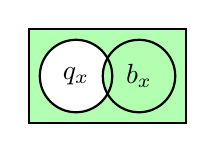
\begin{tikzpicture}[scale=2,fill=green!30,thick]
\def\circ#1#2{(#1,0.3) #2 circle (0.23)}
\def\ca#1{\circ{0.3}{#1}}
\def\cb#1{\circ{0.7}{#1}}
\def\rect{(0,0) rectangle (1,0.6)}
\fill[even odd rule] \rect \ca{}; \fill \cb{};
\draw \rect; \draw \ca{node{$q_x$}}; \draw \cb{node{$b_x$}};
\end{tikzpicture}
\caption{Weakest precondition of \textbf{assume} statements}
\label{fig:wp.assume}
\end{figure}

\paragraph{Assertions} If the statement~$x$ is
\textbf{assert}~$q_x$, then according to condition~2 of
Theorem~\ref{th:correctness} the predicate
\begin{equation}
a_x \limp (q_x \land b_x)
\label{eq:spwp.assertcond}
\end{equation}
must be valid.

In the strongest postcondition method we must find the strongest
predicate~$b_x$, given the predicates $a_x$~and~$q_x$. No matter
what predicate~$b_x$ we choose, the predicate in~\eqref{eq:spwp.assertcond}
is invalid unless
\begin{equation}
a_x \limp q_x
\end{equation}
is valid. If this condition holds, then the strongest
predicate~$b_x$ that satisfies~\eqref{eq:spwp.assertcond} is
\begin{equation}
b_x \equiv (a_x \land q_x).
\end{equation}
In the weakest precondition method we must find the weakest
predicate~$a_x$, given predicates $q_x$~and~$b_x$. 
\begin{equation}
a_x \equiv (q_x \land b_x)
\end{equation}

\paragraph{Assignment} If statement~$x$ is $v:=e$, then according to
condition~2 of Theorem~\ref{th:correctness} the predicate
\begin{equation}
a_x \limp (v \gets e)\;b_x
\label{eq:spwp.assgncond}
\end{equation}
must be valid.

In the strongest postcondition method we must find the strongest
predicate~$b_x$, given the predicate~$a_x$, the variable~$v$, and
the expression~$e$. We rewrite condition~\eqref{eq:spwp.assgncond}.
\begin{equation}
\forall\sigma,\; a_x\;\sigma \limp b_x\;((v\gets e)\;\sigma)
\label{eq:spwp.assgncond2}
\end{equation}
Note that $(v \gets e)\;\sigma=(v\gets e)\;\sigma'$
does not imply $\sigma=\sigma'$. That is, there might be multiple
stores~$\sigma$ corresponding to the same right hand side
in~\eqref{eq:spwp.assgncond2}. Because we want the set~$b_x$ to
be as small as possible we want $b_x\;\sigma$ to hold only if it
must hold, that is, only if there is some corresponding left hand
side in~\eqref{eq:spwp.assgncond2} that holds.
\begin{equation}
b_x\;\sigma = \exists\sigma',\;a\;\sigma' \land
  \bigl( \sigma=(v\gets e)\;\sigma' \bigr)
\end{equation}
It is possible to rewrite this with a quantification
over values instead of the quantification over stores
(see~\eqref{eq:sp-of-assgn}), but since any expression using the
existential quantifier is useless in practice (because of the
limitations of the theorem prover) it makes little sense to spend
more time refining this equation.

In the weakest precondition method we must find the weakest
predicate~$a_x$, given the variable~$v$, the expression~$e$,
and the predicate~$b_x$. This is trivial.
\begin{equation}
a_x \equiv (v\gets e)\;b_x
\end{equation}

\subsection{Summary}
\label{sec:spwp.summary}

In the strongest postcondition method we compute
\begin{align}
a_y &\equiv 
  \begin{cases}
  \tru & \text{if $y$ is the initial statement} \\
  \bigvee_{x \to y} & \text{otherwise}
  \end{cases} \label{eq:spwp.sp.pre}\\
b_x &\equiv
  \begin{cases}
  a_x \land q_x & \text{if $x$ is \textbf{assert}/\textbf{assume}~$q_x$} \\
  \lambda\sigma.\; \exists\sigma',\;a\;\sigma' \land
    \bigl( \sigma=(v\gets e)\;\sigma' \bigr)
    & \text{if $x$ is $v:=e$}
  \end{cases}
  \label{eq:spwp.sp.post}
\end{align}
and we check the validity of
\begin{equation}
\mathit{vc}_\mathit{sp} \equiv \bigwedge_{
  \genfrac{}{}{0pt}{}{\text{$x$ is an}}{text{assertion}} }
  (a_x \limp b_x). \label{eq:spwp.sp.vc}
\end{equation}

In the weakest precondition method we compute
\begin{align}
b_x &\equiv \bigwedge_{x \to y} a_y &  \label{eq:spwp.wp.post}\\
a_x &\equiv 
  \begin{cases}
  q_x \limp b_x &\text{if $x$ is \textbf{assume}~$q_x$}\\
  q_x \land b_x &\text{if $x$ is \textbf{assert}~$q_x$}\\
  (v\gets e)\;b_x &\text{if $x$ is $v:=e$}
  \end{cases}
  \label{eq:spwp.wp.pre}
\end{align}
and we check the validity of
\begin{equation}
\mathit{vc}_\mathit{wp}\equiv a_0.  \label{eq:spwp.wp.vc}
\end{equation}

Equations \eqref{eq:spwp.sp.post}~and~\eqref{eq:spwp.wp.pre}
can be seen as defining the predicate transformer~\textit{sp} and,
respectively, the predicate transformer~\textit{wp}. Both take two
arguments, a statement and a predicate, and return a predicate.


\begin{example}
Let us look again at the program in Figure~\ref{fig:passive-form}
on page~\pageref{fig:passive-form}. The two methods described
above yield equivalent but structurally different VCs:
\begin{equation}
\begin{split}
\mathit{vc}_\mathit{sp} \equiv
  &\big((\tru\land(v_0=u)\land\lnot\mathit{even}(v_0)\land(v_1=v_0+1))\\
  &\lor(\tru\land(v_0=u)\land\mathit{even}(v_0)\land(v_1=v_0))\big)\\
  &\limp\mathit{even}(v_1)
\end{split}\label{eq:vcsp}
\end{equation}
\begin{equation}
\begin{split}
\mathit{vc}_\mathit{wp} \equiv
  &(v_0=u)\limp\\
  &\big((\lnot\mathit{even}(v_0)\limp(v_1=v_0+1)\limp(\mathit{even}(v_1)\land\tru))\\
  &\land(\mathit{even}(v_0)\limp(v_1=v_0)\limp(\mathit{even}(v_1)\land\tru))\big)
\end{split}
\end{equation}
\end{example}
%}}} sec:predicate_transformers
%{{{ sec:theory
\section{Theory}
\label{sec:ra.theory}

Semantic reachability analysis is performed after passivation
(Chapter~\ref{ch:passive}), so the program it analyzes is an
acyclic flowgraph without assignments.

\begin{definition}
A node~$x$ in a flowgraph is \emph{semantically reachable}
when the flowgraph has an execution containing the
state~$\langle\sigma,x\rangle$ for some store~$\sigma$.
\end{definition}

For a correct flowgraph (see Theorem~\ref{th:correctness} on
page~\pageref{th:correctness}), a node~$x$ is semantically
reachable when the flowgraph becomes incorrect after replacing
the statement of node~$x$ with \textbf{assert false}. (This
is because according to~\eqref{eq:assert-nok-opsem} on
page~\pageref{eq:assert-nok-opsem} there is a transition
$\langle\sigma,x:\mathbf{assert}\;\mathbf{false}\rangle\leadsto
\mathit{error}$ for all stores~$\sigma$.) A naive algorithm for
semantic reachability analysis replaces each statement in turn by
\textbf{assert false} and reverifies the program. However, this
algorithm handles only correct flowgraphs and is slow.

There is a very easy way to make any flowgraph correct: Transform
all assertions into assumptions! Besides fixing all bugs, this
transformation has the useful property that it maintains semantic
reachability.

\begin{proposition}
Consider a flowgraph~$G$ with no assignments and the
flowgraph~$H$ obtained by replacing each statement
\textbf{assert}~$q$ with the statement \textbf{assume}~$q$.
Node~$y$ is semantically reachable in flowgraph~$G$ if and only
if it is semantically reachable in flowgraph~$H$.
\end{proposition}

\begin{proof}
According the operational semantics of core Boogie 
(see Chapter~\ref{ch:boogie},
especially~\eqref{eq:assume-assert-ok-opsem}),
a flowgraph has an execution \[
  \langle\sigma,x_1:\mathbf{assert}/\mathbf{assume}\;p_1\rangle,\ldots,
  \langle\sigma,x_n:\mathbf{assert}/\mathbf{assume}\;p_n\rangle,
  \langle\sigma,y\rangle
\] when there is a path $x_1\to\cdots\to x_n\to y$ in the
flowgraph and there is a store~$\sigma$ that satisfies 
$p_1\land\ldots\land p_n$. It is irrelevant whether 
intermediate statements are assertions or assumptions
as there is only one rule in the operational semantics
for both.
\end{proof}

There is still the issue of efficiency.
Chapter~\ref{ch:spwp} showed that both
$\mathit{vc}_\mathit{wp}$~and~$\mathit{vc}_\mathit{sp}$ can be
computed in time linear in the size of the flowgraph. Since we
need to reverify the program once for each node in the flowgraph,
the total time to compute the prover queries is quadratic in
the size of the program. Most flowgraphs in practice have at
most hundreds of nodes and hundreds of edges, which means that a
quadratic algorithm will be very fast and the real problem is the
time spent in the prover.

The next section is concerned with reducing the number of calls
to the prover. Before that, let us briefly see how to compute
\emph{all} prover queries at once in linear time.

If there is an execution that contains the
state~$\langle\sigma,y\rangle$, then the previous
states~$\langle\sigma,x\rangle$ correspond to nodes~$x$ that have
a path~$x\leadsto y$ to node~$y$. Hence, to determine whether
such executions exist we can look at the sub-flowgraph induced by
nodes~$x$ that can reach node~$y$. This observation speeds the
computation of VCs by a factor of two, for both methods---weakest
precondition and strongest postcondition.

Observe now that the precondition~$a_y$ computed by the strongest
postcondition method (Section~\ref{sec:spwp.summary}) depends
only on nodes~$y$ that can reach node~$x$. In other words, the
precondition~$a_y$ does not change when we select a sub-flowgraph
corresponding to some other node~$x'$, so it needs not be
recomputed. We simply compute all preconditions~$a_x$ in
linear time according to the equations for the strongest
postcondition method in Section~\ref{sec:spwp.summary}. When
we replace statement~$x$ by \textbf{assert false} it becomes
the only assertion in the flowgraph and the VC according
to~\eqref{eq:spwp.sp.vc} is $\lnot a_x$. We proved the
following.

\begin{proposition}
A node~$x$ is semantically reachable if and only if its
precondition~$a_x$ computed using the strongest postcondition
method (Chapter~\ref{ch:spwp}) is satisfiable, that is, when
$|\lnot a_x|$ holds.
\end{proposition}

According to~\eqref{eq:spwp.sp.post} (on
page~\pageref{eq:spwp.sp.post}) there is no difference
between \textbf{assume} and \textbf{assert} when computing
preconditions~$a_x$ and postconditions~$b_x$ using the strongest
postcondition method. So one advantage of the strongest
postcondition method is that we do not have to transform
assertions into assumptions at all. Another clear advantage of
the strongest postcondition method is that it produces all prover
queries in linear time, as opposed to the weakest precondition
method which requires quadratic time. It is intuitive that `going
forward' is better suited for analyzing semantic reachability.

\paragraph{Types of Problems} 

Nodes that are semantically unreachable are likely
to be caused by bugs. For example, the contradictory
preconditions in Figure~\ref{fig:ra-bad-spec-ex} (on
page~\pageref{fig:ra-bad-spec-ex}) cause the body of
method~\textit{m2} to be semantically unreachable. It is
therefore interesting to find potential causes of unreachable
code.

A node~$x$ is a \emph{blocker} when it is reachable but lets
no execution pass through it. That is, there is no execution
containing $\langle\_,x\rangle,\langle\_,\_\rangle$. Yet in other
words, the only possible successor of state~$\langle\_,x\rangle$
(in an execution) is the \textit{error} state. If the only
predecessor of node~$y$ is a blocker, then node~$x$ is
semantically unreachable, according to~\eqref{eq:spwp.sp.pre} (on
page~\pageref{eq:spwp.sp.pre}).

There are three types of problems detected by the semantic
reachability analysis:
\begin{enumerate}
\item 
  Semantically unreachable nodes. This includes all dead code.
\item
  Blocker assumptions. These are likely root causes for
  semantically unreachable nodes, so they point closer to
  the actual bug.
\item
  Blocker assertions, also known as doomed program points.
  These are bugs that manifest in every execution.
\end{enumerate}

Formally, there can be no error after a blocker. That is, there
is no execution that goes wrong after it passed through a
blocker, for the simple reason that there is no execution passing
through a blocker. However, intuitively it is helpful to think of
blockers as potentially hiding subsequent bugs.
%}}} sec:theory
%{{{ sec:algorithm
\section{Algorithm}

Figure~\ref{fig:ra.naive_alg} summarizes the algorithm
suggested by the previous section. The methods \textit{Pre}
and \textit{Post} are those from Figure~\ref{fig:sp-algo} (on
page~\pageref{fig:sp-algo}); the method $\mathit{Not}(p)$
constructs the SMT dag that represents the predicate~$\lnot
p$, perhaps carrying out basic simplifications; the method
\textit{Valid} checks whether its argument represents a valid
predicate by querying the prover. The $|V|$ calls to the method
\textit{Pre} take $O(|V|+|E|)$ time and similarly for method
\textit{Post} (see the proof of Proposition~\ref{prop:sptime} on
page~\pageref{prop:sptime}).

%{{{fig:ra.naive_alg
\begin{figure}\centering\leavevmode\vbox{
\begin{alg}
\^  $\proc{NaiveReachabilityAnalysis}(G)$
\=  ~for~ ~each~ statement $x$ of $G$
\+    ~if~ $\mathit{Valid}(\mathit{Not}(\mathit{Pre}(x)))$
\+      report that node $x$ is semantically unreachable
\-    ~if~ statement $x$ is an assertion ~and~ $\mathit{Valid}(\mathit{Not}(\mathit{Post}(x)))$
\+        report that node $x$ is doomed
\end{alg}}
\caption{A simple algorithm for semantic reachability analysis}
\label{fig:ra.naive_alg}
\end{figure}
%}}}

This algorithm reports too many errors. For the Boogie program
\begin{boogie}
assume false;
assert $p_1$;
$\cdots$
assert $p_n$;
\end{boogie}
it prints $n$~error messages, one for each assertion. Surely,
the user would prefer one error message that points at the
assumption, which is the cause of all the other errors.

More seriously, it turns out that this algorithm, even if it
takes just linear time to build the prover queries, is unusable
in practice because it is too slow. It is simply not acceptable
to call the prover $|V|$~times for one method. A typical method
has $|V|\approx100$ nodes, and one call to the prover typically
takes between a tenth of a second and one second.

\begin{remark}
All the times are given for an implementation inside \escjava,
which is activated by the option~\texttt{-era}. \escjava has a
robust frontend for Java with JML annotations, so it is easier
to perform meaningful experiments. The implementation first
constructs a flowgraph essentially equivalent to those built by
FreeBoogie, so the implementation should be easy to adapt.
\end{remark}

\subsection{The Propagation Rules}

Figure~\ref{fig:fg.chain.a} shows a path flowgraph. (Node~$1$ is
the initial node.) Node~$4$ is semantically reachable when there
is an execution that contains the state~$\langle\sigma,4\rangle$,
for some store~$\sigma$. Such an execution must correspond
to some path from the initial node~$1$ to node~$4$, and the
only such path is $1\to2\to3\to4$. Hence, the execution
is $\langle\sigma,1\rangle$,~$\langle\sigma,2\rangle$,
$\langle\sigma,3\rangle$, $\langle\sigma,4\rangle$, which means
that the other nodes are semantically reachable too. (The store
is not modified by assertions or assumptions.) This motivates the
study of the following problem, which is more abstract.

%{{{fig:fg.chain
\begin{figure}
\def\sf#1#2#3{
  \subfigure[]{\label{fig:fg.chain.#1}
    \begin{tikzpicture}
    \foreach \n in {#2}
      \enode (\n) at (0,-\n) [label=right:$\n$] {};
    \foreach \n in {#3}
      \fnode (\n) at (0,-\n) [label=right:$\n$] {};
    \draw (1)--(2)--(3)--(4);
    \end{tikzpicture}
  }
}
\centering
\sf a{1,2,3,4}{}\hfil
\sf b{1,2,3}{4}\hfil
\sf c{1,2}{3,4}\hfil
\sf d{1}{2,3,4}\hfil
\sf e{}{1,2,3,4}
\caption{A path flowgraph with $4$ nodes}
\label{fig:fg.chain}
\end{figure}
%}}}

\begin{problem}
Alice and Bob play a game. They start by sharing the
flowgraph~$G$. Then Alice secretly colors the nodes with white
and black such that each white node is connected by a white path
with the initial node. Bob's goal is to reconstruct the coloring
by asking Alice as few questions as possible. He is allowed to
ask ``what is the color of node~$x$?''\ for any node~$x$ and
Alice will answer truthfully.
\label{pb:ra.abstract}
\end{problem}

\begin{remark}
Alice is the theorem prover, Bob is FreeBoogie (or \escjava),
white nodes are semantically reachable nodes, and black nodes are
semantically unreachable nodes.
\end{remark}

Bob's flowgraph initially has only gray nodes and, by the end,
he colors each with either white or black. At some intermediary
stage, he has some white nodes, some black nodes, and the rest
are gray. We say that two colorings are \emph{consistent} when
there is no node that is white in one coloring and black in
the other. Bob maintains his coloring consistent with Alice's
coloring. (Also, because it is not useful, he never changes the
color of a node into gray.) A \emph{valid coloring} has no gray
node and satisfies the condition that
\begin{equation}
\label{eq:ra.fg-cond}
\text{every white node is reachable from the initial node 
by a white path.}
\end{equation}
For example, Figure~\ref{fig:fg.chain} shows all the valid
colorings of a path flowgraph. A \emph{possible coloring} (at
some intermediate stage) is a valid coloring that is consistent
with Bob's coloring. The rule which Bob uses to paint nodes
white or black is simple: If node~$x$ is white in all possible
colorings, then Bob colors it white; if node~$x$ is black in
all possible colorings, then Bob colors it black. Obviously,
this maintains the invariant that Bob's coloring is consistent
with Alice's coloring. To ensure progress, Bob asks Alice from
time to time about the color of a node that is still gray in his
coloring.

\begin{example}
Consider the flowgraph in Figure~\ref{fig:ra.fg.worst}. The
initial node is always reachable. Assuming that Bob starts
with the initial node white and the others gray, he must ask
$5$~questions. After asking $k$~questions he must consider
$2^{5-k}$ possible colorings. However, the preconditions of
all non-initial nodes are the same as the postcondition of
the initial node. Therefore, they are either all semantically
reachable or all semantically unreachable, and this can be
determined with one call to the prover.
\label{ex:ra.bad-model}
\end{example}

\begin{figure}\centering
\begin{tikzpicture}
\enode (r) at (0,1) {};
\foreach \x in {-2,-1,...,2} {
  \gnode (\x) at (\x,0) {};
  \draw (r)--(\x);
}
\end{tikzpicture}
\caption{Worst case flowgraph}
\label{fig:ra.fg.worst}
\end{figure}

Example~\ref{ex:ra.bad-model} seems to suggest that performance
is hurt because Problem~\ref{pb:ra.abstract} is a \emph{too}
abstract model. Related to this, it seems that the theorem
prover is never queried about doomed code (unsatisfiable
postconditions), but only about semantically unreachable code
(unsatisfiable preconditions). Both these issues have an
easy fix. Instead of playing the color game on the original
flowgraph, Alice and Bob play it on a modified flowgraph
that has two nodes $x_i$~and~$x_o$ for each node~$x$ in the
original flowgraph. Node~$x_i$ takes over the incoming edges
of node~$x$; node~$x_o$ takes over the outgoing edges of
node~$x$. Also, there is an edge~$x_i\to x_o$. When Bob asks
Alice about the color of node~$x_i$, this means that \escjava
(or FreeBoogie) asks the theorem prover about the satisfiability
of the precondition~$a_x$; when Bob asks Alice about the
color of node~$x_o$, this means that \escjava (or FreeBoogie)
asks the theorem prover about the satisfiability of the
postcondition~$b_x$.

Bob does not want to look at each possible coloring, because
there might be an exponential number of them. Hence, he must
characterize the nodes whose color he can infer without referring
to all possible colorings.

\begin{definition}
Node $x$ of a flowgraph \emph{dominates} node~$y$ when all
paths from the initial node to node~$y$ contain node~$x$.
Node~$x$ \emph{immediately dominates} node~$y$ if $x\ne y$
and all nodes that dominate node~$y$ also dominate node~$x$.
\label{def:ra.dominator}
\end{definition}

\begin{proposition}
A gray node is white in all possible colorings if and only if
it dominates a white node in the non-black subgraph (in Bob's
coloring). \label{prop:ra.fix-white}
\end{proposition}

\begin{proof}
Because Bob's coloring is consistent with a valid coloring it is
possible, for each white node~$y$ to find a non-black path from
the initial node to node~$y$. Consider the coloring constructed
by picking such a path for each white node and then painting all
these paths white; then paint the remaining gray nodes black.
This coloring is possible by construction. Also, whenever white
node~$y$ is processed, choose a path that avoids node~$x$, if
possible. This shows that if node~$x$ does not dominate a white
node, then there are some possible colorings in which it is
black. 

For the converse, consider a coloring in which node~$x$ is black
and dominates white node~$y$. Then \eqref{eq:ra.fg-cond}~is
violated and the coloring is invalid.
\end{proof}

Similarly, one can prove the following.

\begin{proposition}
A gray node~$x$ is black in all possible colorings if and only if
all the paths from the initial node to node~$x$ contain a black
node (in Bob's coloring). \label{prop:ra.fix-black}
\end{proposition}

An immediate consequence of the last two proposition will prove
useful.

\begin{corollary}
A gray node is sometimes white and sometimes black in possible
colorings if and only if in the non-black subgraph (a)~it does
not dominate a white node and (b)~it is connected to the initial
node. (Again, in Bob's coloring.)
\label{co:ra.propagate}
\end{corollary}

Figure~\ref{fig:alg_propagate} shows how Bob paints his
flowgraph. The method \textit{ComputeDominators} computes the
dominator tree of a graph (Section~\ref{sec:ra.dominators}).
The method \textit{PickQueryNode} returns some gray node
(Section~\ref{sec:ra.heuristic}). The main loop of the method
\textit{RecoverColoring} maintains the invariants:
\begin{enumerate}
\item The coloring is consistent with Alice's coloring.
\item 
  For each gray node, there are possible colorings in which
  it is white and possible colorings in which it is black.
\end{enumerate}
It is easy to see that both invariants hold when all the nodes
are gray. Let us see why they are maintained, first in the case
when Alice says that node~$x$ is white and then in the case when
Alice says that node~$x$ is black.

%{{{fig:alg_propagate
\begin{figure}\centering\leavevmode\vbox{
\begin{alg}
\^  $\proc{PropagateWhite}(y, T)$
\=  paint node $y$ in white
\=  \textit{PropagateWhite}(parent of $y$ in tree $T$)
\end{alg}
\bigskip
\begin{alg}
\^  $\proc{PropagateBlack}(x,G)$
\=  paint node $x$ in black
\=  ~for~ ~each~ gray successor $y$ of node $x$ in $G$
\+    ~if~ all predecessors of node $y$ are black
\+      $\mathit{PropagateBlack}(y, G)$
\end{alg}
\bigskip
\begin{alg}
\^  $\proc{RecoverColoring}(G)$
\=  paint in gray all the nodes of the flowgraph $G$
\=  ~while~ there are gray nodes
\+    $T:=\mathit{ComputeDominators}(\text{non-black subgraph of $G$})$
\=    $x:=\mathit{PickQueryNode}(G,T)$
\=    ~if~ $\mathit{AskAlice}(x)=\textit{white}$
\+      $\mathit{PropagateWhite}(x,T)$
\-    ~else~
\+      $\mathit{PropagateBlack}(x,G)$
\end{alg}}
\caption{Solution outline for Problem~\ref{pb:ra.abstract}}
\label{fig:alg_propagate}
\end{figure}
%}}}

If Alice says that node~$x$ is white then there are no possible
colorings in which it is black, so it must be painted white
to maintain invariant~2. This is done on line~1 of the method
\textit{PropagateWhite} when it is first called from line~6
of the method \textit{RecoverColoring}. However, painting
node~$x$ in white might break invariant~2 with respect to
another gray node, because gray nodes must not dominate white
nodes (Corollary~\ref{co:ra.propagate}). This problem is
fixed by painting all the dominators of node~$x$ in white,
which is allowed by Proposition~\ref{prop:ra.fix-white}.
It follows from the definition of an immediate dominator
(Definition~\ref{def:ra.dominator}) that method
\textit{PropagateWhite} visits exactly the dominators of
node~$x$.

If Alice says that node~$x$ is black then, for similar reasons as
in the previous case, it must be painted black. This may break
the other part of invariant~2, namely, it may make disconnect
gray nodes from the initial node in the non-black subgraph.
Should this happen, Proposition~\ref{prop:ra.fix-black} says
that all the disconnected gray nodes must be painted black.
This is the purpose of the method \textit{PropagateBlack}. Let
us say that a node is immediately disconnected when all its
parents are black. Initially no node is immediately disconnected
(invariant~2) but one may become so when its parent is painted
black (on line~1 of the method \textit{PropagateBlack}).
Whenever this happens it will be visited. Therefore, the
method \textit{PropagateBlack} visits and paints in black all
immediately blocked nodes. Now it is easy to see that if all
immediately blocked nodes are black, then there is no gray node
that is disconnected from the initial node in the non-black
subgraph. Pick some gray node. Because it is not black, it is
not immediately blocked, so it has a non-black predecessor. Then
repeat.

We have proved that the algorithm is correct. It is also fast.

\begin{proposition}
If calls $\mathit{ComputeDominators}()$, $\mathit{PickQueryNode}()$,
and $\mathit{AskAlice}()$ each takes constant time, then the method
\textit{RecoverColoring} takes $O(|V|+|E|)$ time.
\end{proposition}

\begin{proof}
The methods \textit{PropagateWhite} and \textit{PropagateBlack}
are called only for gray nodes and the first action paint the
given node in black or white. Therefore, they are called at most
once per node.

The method~\textit{PropagateBlack} examines the outgoing edges of
node~$x$, so it might examine all edges by the end. The condition
on line~3 of the method \textit{PropagateBlack} can be evaluated
in constant time if each node keeps a count of its non-black
parents.
\end{proof}


\subsection{Dominators Tree for Dags}
\label{sec:ra.dominators}

This section is a brief reminder of basic algorithms related to
dominators. It explains how the method \textit{ComputeDominators}
in Figure~\ref{fig:alg_propagate} is implemented.

The dominators tree~$T$ of a flowgraph~$G$ is a tree in which the
parent of node~$x$, denoted $\mathit{idom}(x)$, is the immediate
dominator of node~$x$ in the flowgraph~$G$. The root of the
dominators tree is the initial node of the flowgraph, which is
the only node without an immediate dominator. All other nodes~$y$
obey the equation
\begin{equation}
\mathit{idom}(y)=\mathit{LCA}(\{\,x\mid x\to y\,\}),
\end{equation}
where $\mathit{LCA}(S)$ is the root of the smallest dominators
subtree that contains the set~$S$ of nodes.

The method \textit{ComputeDominators} examines nodes in a
topological order of the flowgraph and inserts them as leafs in
the proper place in the dominators tree that it builds. When
node~$y$ is processed all its predecessors~$x$ have taken their
place in the dominators tree so \textit{LCA} can be computed.


\subsection{Choosing the Query}
\label{sec:ra.heuristic}

A greedy algorithm always asks the query whose answer provides
most information. If the probability of receiving the answer
\textit{black} is~$p$, then the information provided by the
answer is $p\lg p + (1-p)\lg(1-p)$, which has a maximum at
$p=1/2$ and is symmetric around that point. In other words, the
greedy information theoretic approach says that we should always
inquire about the node whose probability of being black is as
close as possible to~$1/2$.

\paragraph{An Example}

To estimate the probability of various nodes being black we
need a model. Let us go back to the example flowgraph in
Figure~\ref{fig:fg.chain} (on page~\pageref{fig:fg.chain}).
The simplest possible model is the one in which each node has
an independent probability~$p$ of having a \emph{bug} and
probability $q=1-p$ of not having a bug. A node with a bug
is black and so are all that follow it. In this model, the
five possible colorings of Figure~\ref{fig:fg.chain} have
probabilities (a)~$q^4$, (b)~$q^3p$, (c)~$q^2p$, (d)~$qp$, and
(e)~$p$. The probability that node~$x$ is black is the sum of
probabilities of possible colorings in which node~$x$ is black.
For the nodes in Figure~\ref{fig:fg.chain} we have (1)~$1-q$,
(2)~$1-q^2$, (3)~$1-q^3$, and (4)~$1-q^4$.

In general, for a path flowgraph with nodes $1\to2\to\cdots\to
n$, the probability that node~$k$ is black is
\begin{equation}
p_k = 1 - (1 - p)^k
\end{equation}
where $p$ is the probability that a node has a bug. In the common
case, we expect the analysis to be run on code that is mostly
correct. Indeed, bugs are usually clustered in the region of the
code that is actively developed, while the program verifier is
run on the whole code base. Hence, in a first approximation, it
is reasonable to expect $p$ to be very small. Then $p_k\approx
kp$ and, if $p$~is really small, the probability that is closest
to~$1/2$ is~$p_n$. In other words, if we are fairly confident
that the code is correct, then we should query the last node in
the path. If the code is indeed correct, then we are done after
one query.

However, if the first query returns \textit{black} then there is
at least one bug. The expected number of bugs for the model we
use is $b=pn$. (The number of bugs has the probability generating
function
\begin{equation}
B(z)=\sum_k \binom{n}{k} (1-p)^{n-k} p^k z^k = (1-p+pz)^n,
\end{equation}
so the average is $B'(1)=pn$.) Therefore, if we expect the
program to have $b$~bugs, then it makes sense to choose
\begin{equation}
p=b/n \label{eq:ra.bug-estim}
\end{equation}
in our model. Solving $p_k=1/2$ we obtain
\begin{equation}
k=-1/\lg(1-p)\approx(\ln2)/p.
\end{equation}
Plugging in the estimate~\eqref{eq:ra.bug-estim} we finally
arrive at
\begin{equation}
k\approx 0.7\cdot n/b
\end{equation}
In other words, the information theoretic greedy strategy is
a binary search that splits the interval~$i.\,.\>j$ not at
$i+0.5(j-i)$, but at $i+(0.7/b)(j-i)$, where $b$ is the expected
number of bugs in the interval~$i.\,.\>j$.

\paragraph{The General Case}

Most observations for path flowgraphs generalize easily. We will
have two modes of work, one in which we expect no bug and one in
which we expect one bug. When we expect no bug we will pick a
gray node that is far from the initial node. When we expect one
bug we will perform a binary search on a path of nodes in the
dominator tree. The key here is that color propagation rules on
paths in the dominator tree are exactly the same as the color
propagation rules for a path flowgraph.

Figure~\ref{fig:ra.alg} summarizes all the observations made
so far. Line~1 splits each node~$x$ of the flowgraph into a
node~$x_i$ carrying the precondition~$a_x$ and a node~$x_o$
carrying the postcondition~$b_x$. Later these predicates are
accessed using the method \textit{Formula}(). Line~2 colors the
initial node white to establish the invariant of the loop on
line~10.

%{{{fig:ra.alg
\begin{figure}\centering\leavevmode\vbox{
\begin{alg}
\^  $\proc{ReachabilityAnalysis}(G)$
\=  construct $H$ by splitting nodes of $G$
\=  paint the initial node of $H$ white and the others gray
\=  $T:=\mathit{ComputeDominators}(H)$
\=  ~while~ $H$ has gray nodes
\+    $x:=\text{a leaf from the deapest level of $T$}$
\=    ~if~ $\mathit{Valid}(\mathit{Not}(\mathit{Formula}(x)))$
\+      $\mathit{PropagateBlack}(x,H)$
\=      let $[y_1,\cdots,y_n]$ be the path in $T$ from $y_1=\mathit{root}(T)$ to $y_n=x$
\=      $i:=1,\quad j:=n$
\=      ~while~ $i+1<j$ \comment $y_i$ is white, $y_j$ is black
\+        $k:=\mathit{round}(i+0.7(j-i))$
\=        ~if~ $\mathit{Valid}(\mathit{Not}(\mathit{Formula}(y_k)))$
\+          $\mathit{PropagateBlack}(y_k, H)$
\=          $j:=k$
\-        ~else~
\+          $\mathit{PropagateWhite}(y_k, T)$
\=          $i:=k$
\2      $T:=\mathit{ComputeDominators}(\text{non-black subgraph of $H$})$
\-    ~else~
\+      $\mathit{PropagateWhite}(x,T)$
\end{alg}
}
\caption{Algorithm for semantic reachability analysis}
\label{fig:ra.alg}
\end{figure}
%}}}

\subsection{Performance}

If the verified flowgraph has no bugs (no semantically
unreachable statements and no doomed code) then $l$~queries are
necessary and sufficient, where $l$~is the number of leafs in
the flowgraph. The algorithm reaches this bound. In other words,
if there are no bugs, then the prover is queried once for each
\textbf{return} statement in the program. For each bug, there are
$\sim\lg h$ extra queries, where $h$~is the (average) length of a
path in the flowgraph from the initial node to a \textbf{return}
node. In total, there are roughly $l+b\lg h$ queries for a
program with $b$~bugs.

\paragraph{Experiments}

The frontend of \escjava (JavaFE) contains $1890$~methods and is
one of the largest coherent JML-annotated code base. Verifying
it takes $31589$~seconds (almost $9$~hours), out of which
$34.8\%$~is spent in semantic reachability analysis, out of
which $99.8\%$~is spent in the prover. The total number of leafs
in flowgraphs is~$3256$ and the total number of prover queries
is~$3351$. In other words, on average per method
\begin{itemize}
\item 
  semantic reachability analysis takes $5.82$~seconds,
\item 
  out of which $5.81$~seconds are spent in $1.77$ prover queries
  (not much more than the number of \textbf{return} statements, which
  is~$1.72$)
\item
  and the other $0.01$~seconds are spent computing prover
  queries, deciding which queries to perform, and propagating
  semantic reachability information in the flowgraph.
\end{itemize}
(This benchmark was run using the default treatment of loops in
\escjava---unrolling once.)
%}}} sec:algorithm
%{{{ sec:case_study
\section{Case Study}
\label{sec:ra.case_study}

The frontend of \escjava (known as JavaFE) consists of
$217$~annotated classes with $1890$~methods. Semantic
reachability analysis revealed $\approx50$~issues. Short
descriptions of these problems follow, each description preceded
by the number of cases to which it applies.

\subsection{Dead Code}

\begin{itemize}
\item[1] 
  A \textbf{catch} block was unreachable because it was catching
  a \textit{RuntimeException} and the specifications of methods
  called in the \textbf{try} block did not signal that exception type.
\item[9]
  Informal comments indicated that the dead code is intended.
  JML has an equivalent annotation, which \escjava understands
  and should be used instead of the informal comments.
\item[1]
  The code was semantically unreachable in the classic sense (no
  annotation involved.)
\end{itemize}

\subsection{Doomed Code}

\begin{itemize}
\item[6] A few assertions were bound to fail on any input.
\item[9]
  The scenario illustrated by methods \textit{m2}~and~\textit{m3}
  in Figure~\ref{fig:ra-doomed-code-ex} on
  page~\pageref{fig:ra-doomed-code-ex}. The method call
  was bound to fail.
\end{itemize}

\subsection{Inconsistent Specifications}

\begin{itemize}
\item[5] 
  Inconsistencies in the JDK specifications that ship with
  \escjava. They were filed as \escjava bugs \#595, \#550, \#568,
  \#549, and \#545. These are bugs whose cause was hard to track.
  Before, they have escaped for years the \escjava's test-suite 
  that was designed to catch them.
\end{itemize}

\subsection{Unsoundness and Bugs}

\begin{itemize}
\item[1]
  The JDK specification used a JML \emph{informal comment}.
  According to the semantics of JML, an informal comment should
  not cause warning messages. Roughly, this means that, depending
  on the context, an informal comment should be treated sometimes
  as \textbf{true} and sometimes as \textbf{false}. However,
  \escjava always treats is as \textbf{true}. See \escjava bug
  \#547 for details.
\item[4]
  Loops with a constant bound that is bigger than the loop 
  unrolling limit.
\item[2]
  If the \textbf{modifies} clause is missing on a method~$m$,
  \escjava considers that method~$m$ is allowed to modify any
  global variable while checking it, but assumes that method~$m$
  does not modify any global state while checking methods that
  call it. This is obviously unsound (and motivated by the desire
  to not flood new users with irrelevant warnings).
\end{itemize}

\subsection{Others}

\begin{itemize}
\item[12] 
  The cause of these warnings provided by the semantic
  reachability analysis is unclear. Given the experience of
  tracking down the cause of some of the other warnings, it is
  likely that a complex interaction between annotations located
  in different files is involved.
\end{itemize}
%}}} sec:case_study
%{{{ sec:conclusions
\section{Conclusions and Related Work}
\label{sec:ra.conclusions}

This chapter presents the theoretical underpinnings of semantic
reachability analysis for annotated code and an efficient
algorithm for finding 
\begin{enumerate}
\item dead code,
\item doomed code,
\item inconsistent specifications, and
\item unsoundness bugs.
\end{enumerate}

% Dead

Abstract interpretation~\cite{cousot1977} and symbolic
execution~\cite{king1976} are program verification techniques
that can easily detect semantically unreachable code as a
by-product, although they seldom seem to be used for this
purpose. To ensure termination, these techniques usually
over-approximate the set of possible states, which means that
they might conclude that some code is semantically reachable,
although it is not.

Lermer et al.~\cite{lermer2003} give semantics for execution
paths using predicate transformers. In particular, they define
\emph{dead paths} and \emph{dead commands}. A dead path is one
that is taken by no execution; a dead command is a program whose
VC computed by the weakest precondition method is unsatisfiable.

% Doomed

Hoenicke et al.~\cite{hoenicke2009} explain why it is desirable
to detect doomed code. Their implementation uses the weakest
precondition method to compute prover queries associated with
each node. The irrelevant portions of the flowgraph are turned
off using auxiliary variables rather than explicitly manipulating
the flowgraph (see Section~\ref{sec:ra.theory}).

% Inconsistent

Chalin~\cite{chalin2006} explains why it is desirable to have
automatic sanity checks for specifications and designs an
automated analysis that finds bugs in JML annotations, other than
plain logic inconsistencies.

Cok and Kiniry~\cite{cok2005methods,cok2004} explain how
\escjava handles method calls that appear in annotations. Darvas
and M\"uller~\cite{darvas2006methods} point out that that
treatment is unsound because some annotations are translated
by \escjava's frontend into inconsistent assumptions. Their
solution is a set of syntactic constraints on the use of
method calls in annotations. Rudich et al.~\cite{rudich2008}
relax these constraints while maintaining soundness. Leino and
Middelkoop~\cite{leino2009methods} replace the syntactical
constraints with queries to the theorem prover. Semantic
reachability analysis will signal most problems caused by the
use of method calls in specification, because they manifest as
inconsistencies at the level of the intermediate representation
(Boogie). In particular, it is similar to the approach of Leino
and Middelkoop~\cite{leino2009methods} in its use of a theorem
problem. However, being a generic analysis, the error message is
usually not very informative. Another shortcoming of the semantic
reachability analysis compared to the other specialized solutions
is that it does not ensure that specifications are well-founded.

% Bugs

The naive version of semantic reachability analysis is used in
the static verifier Boogie from Microsoft Research under the name
``smoke testing'' and is used mostly for catching bugs in the
verifier itself.

% Background

\escjava~\cite{flanagan2002escjava} is a program verifier for
Java annotated with JML~\cite{leavens2006jml,cok2004}. By design,
\escjava favors user friendliness over soundness.

The method \textit{ComputeDominators} uses the algorithm of
Cooper~\cite{cooper2000}, which is easy to implement and
works fast in practice~\cite{georgiadis2006}. (There are
linear time algorithms, such as the one of Buchsbaum et
al.~\cite{buchsbaum2008}.) Probability generating functions,
such as the one used in Section~\ref{sec:ra.heuristic}, are
treated by most probability textbooks, such as Graham et
al.~\cite[Chapter~8]{graham1998}.
%}}} sec:conclusions


\bibliographystyle{plain}
\bibliography{semantic_reachability}

\end{document}
% vim:spell errorformat=%f\:%l-%m,%f\:%l\:%m,%f\:%m

